\documentclass{standalone}
\usepackage{graphicx}	
\usepackage{amssymb, amsmath, amsthm}
\usepackage{color}

\usepackage{tikz}
\usetikzlibrary{intersections, backgrounds, math, decorations.pathreplacing}

\definecolor{light}{RGB}{220, 188, 188}
\definecolor{mid}{RGB}{185, 124, 124}
\definecolor{dark}{RGB}{143, 39, 39}
\definecolor{highlight}{RGB}{180, 31, 180}
\definecolor{darkteal}{RGB}{29, 79, 79}
\definecolor{darkolive}{RGB}{97, 123, 45}
\definecolor{gray10}{gray}{0.1}
\definecolor{gray20}{gray}{0.2}
\definecolor{gray30}{gray}{0.3}
\definecolor{gray40}{gray}{0.4}
\definecolor{gray60}{gray}{0.6}
\definecolor{gray70}{gray}{0.7}
\definecolor{gray80}{gray}{0.8}
\definecolor{gray90}{gray}{0.9}
\definecolor{gray95}{gray}{0.95}

\begin{document}

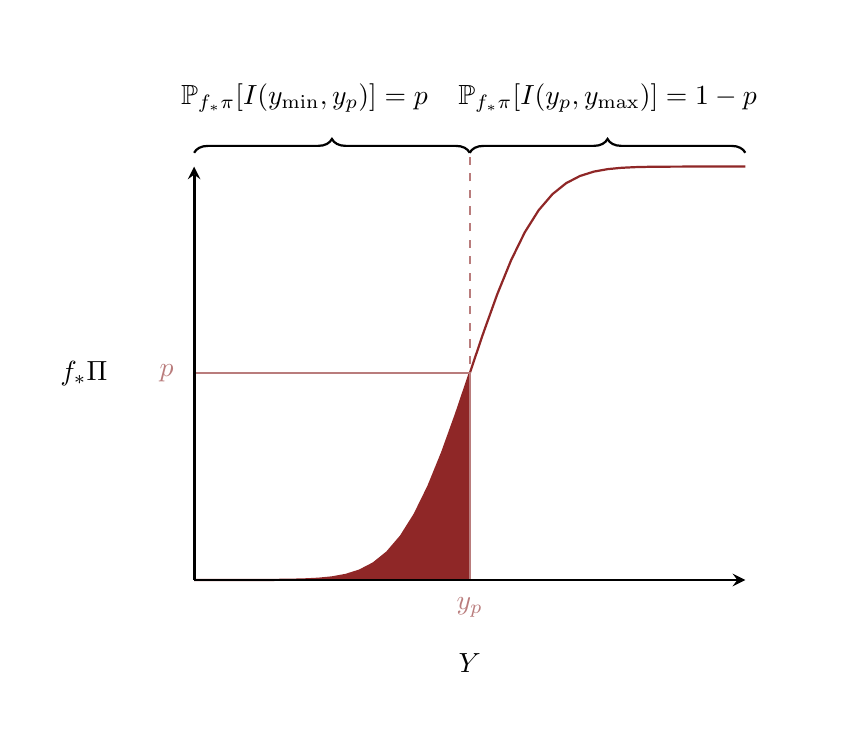
\begin{tikzpicture}[scale=0.35, thick]
 
\begin{scope}[shift={(0, -24)}]
  \draw[white] (-6, -5) rectangle (23, 20);
  
  \begin{scope}
    \clip (0, 0) rectangle (10, 11);
  \fill[dark] (0.0, 0)
-- (0.5, 1.525625e-05)
-- (1.0, 5.096510e-05)
-- (1.5, 1.603279e-04)
-- (2.0, 4.750686e-04)
-- (2.5, 1.326259e-03)
-- (3.0, 3.489436e-03)
-- (3.5, 8.655376e-03)
-- (4.0, 2.024847e-02)
-- (4.5, 4.469645e-02)
-- (5.0, 9.314498e-02)
-- (5.5, 1.833671e-01)
-- (6.0, 3.412520e-01)
-- (6.5, 6.008874e-01)
-- (7.0, 1.002108e+00)
-- (7.5, 1.584747e+00)
-- (8.0, 2.379829e+00)
-- (8.5, 3.399410e+00)
-- (9.0, 4.628063e+00)
-- (9.5, 6.019405e+00)
-- (10.0, 7.500000e+00)
-- (10.5, 8.980595e+00)
-- (11.0, 1.037194e+01)
-- (11.5, 1.160059e+01)
-- (12.0, 1.262017e+01)
-- (12.5, 1.341525e+01)
-- (13.0, 1.399789e+01)
-- (13.5, 1.439911e+01)
-- (14.0, 1.465875e+01)
-- (14.5, 1.481663e+01)
-- (15.0, 1.490686e+01)
-- (15.5, 1.495530e+01)
-- (16.0, 1.497975e+01)
-- (16.5, 1.499134e+01)
-- (17.0, 1.499651e+01)
-- (17.5, 1.499867e+01)
-- (18.0, 1.499952e+01)
-- (18.5, 1.499984e+01)
-- (19.0, 1.499995e+01)
-- (19.5, 1.499998e+01)
-- (20.0, 1.500000e+01)
-- (20.0, 0);
  \end{scope}
  
    \draw[dark] (0.0, 0)
-- (0.5, 1.525625e-05)
-- (1.0, 5.096510e-05)
-- (1.5, 1.603279e-04)
-- (2.0, 4.750686e-04)
-- (2.5, 1.326259e-03)
-- (3.0, 3.489436e-03)
-- (3.5, 8.655376e-03)
-- (4.0, 2.024847e-02)
-- (4.5, 4.469645e-02)
-- (5.0, 9.314498e-02)
-- (5.5, 1.833671e-01)
-- (6.0, 3.412520e-01)
-- (6.5, 6.008874e-01)
-- (7.0, 1.002108e+00)
-- (7.5, 1.584747e+00)
-- (8.0, 2.379829e+00)
-- (8.5, 3.399410e+00)
-- (9.0, 4.628063e+00)
-- (9.5, 6.019405e+00)
-- (10.0, 7.500000e+00)
-- (10.5, 8.980595e+00)
-- (11.0, 1.037194e+01)
-- (11.5, 1.160059e+01)
-- (12.0, 1.262017e+01)
-- (12.5, 1.341525e+01)
-- (13.0, 1.399789e+01)
-- (13.5, 1.439911e+01)
-- (14.0, 1.465875e+01)
-- (14.5, 1.481663e+01)
-- (15.0, 1.490686e+01)
-- (15.5, 1.495530e+01)
-- (16.0, 1.497975e+01)
-- (16.5, 1.499134e+01)
-- (17.0, 1.499651e+01)
-- (17.5, 1.499867e+01)
-- (18.0, 1.499952e+01)
-- (18.5, 1.499984e+01)
-- (19.0, 1.499995e+01)
-- (19.5, 1.499998e+01)
-- (20.0, 1.500000e+01);

  \draw[mid, dashed] (10, 0) -- (10, 15.5);
  \draw[mid] (0, 7.5) -- (10, 7.5) -- (10, 0);
  \node[mid] at (-1, 7.5) { $p$ };
  \node[mid] at (10, -1) { $y_{p}$ };
  
  \draw[decorate,decoration={brace,amplitude=5pt}] (0, 15.5) -- (10, 15.5);
  \node at (4, 17.5) { $\mathbb{P}_{f_{*} \pi}[I( y_{\text{min}}, y_{p} )] = p$ };

  \draw[decorate,decoration={brace,amplitude=5pt}] (10, 15.5) -- (20, 15.5);
  \node at (15, 17.5) { $\mathbb{P}_{f_{*} \pi}[I( y_{p}, y_{\text{max}} )] = 1 - p$ };
  
  \draw[->, >=stealth, line width=1] (0, 0) -- (20, 0);
  \node at (10, -3) { $Y$ };
  
  \draw[->, >=stealth, line width=1] (0, 0) -- (0, 15);
  \node at (-4, 7.5) { $f_{*} \Pi$ };
  
\end{scope}

\end{tikzpicture}

\end{document}  